\documentclass{beamer}
\usepackage[utf8]{inputenc}
\usepackage{graphicx}
\author[Sowmya Vajjala]{Instructor: Sowmya Vajjala}

\title[LING 410X]{LING 410X: Language as Data}
\subtitle{Semester: Spring '18}

\date{3 Apr 2018}

\institute{Iowa State University, USA}
%%%%%%%%%%%%%%%%%%%%%%%%%%%

\begin{document}

\begin{frame}\titlepage
\end{frame}

\begin{frame}
\frametitle{Class Outline}
\begin{itemize}
\item Announcement about: Extension for Assignment 5
\item Text visualization: Overview
\item Assignment 6 description
\end{itemize}
\end{frame}

\begin{frame}
\frametitle{Announcement}
\begin{itemize}
\item I asked IT support to install mallet on all lab computers. They said they will do it today.
\item For those using topicmodels library: Check the discussion forum "Any general R question you want to ask", there is  a potential solution for the problems you are facing.
\item All of you get an extension until the end of this week to submit this Assignment, without any penalty.
\item Those who already submitted need not submit again. 
\end{itemize}
\end{frame}

\begin{frame}
\frametitle{}
\centering
\Large Text visualization: Overview
\end{frame}

\begin{frame}
\frametitle{What is "text visualization" for us?}
\framesubtitle{Disclaimer}
\begin{itemize}
\item We are talking about ways to visualize textual data to summarize some analysis about the text, or summarize the text itself.
\item We are not talking about font design, webpage layout, usage of font sizes, italics etc.
\end{itemize}
\end{frame}


\begin{frame}
\frametitle{Why visualize?}
To get a quick summary about data, for different purposes:
\begin{itemize}
\item showing/summarizing content of a single text
\item showing similarity between texts 
\item showing opinions/emotions/sentiment about something (e.g., using tweets)
\item general exploration of textual data
\end{itemize}
\footnotesize source: Introduction to Text Visualization by Nan Cao and Weiwei Cui, Springer (available online for free from ISU network).
\end{frame}

\begin{frame}
\frametitle{Why visualize?: Some application scenarios}
\framesubtitle{Knowing what are the important/frequent words in a document}
\includegraphics[width=0.99\textwidth]{wordcloud.png} \\
\end{frame}

\begin{frame}
\frametitle{Why visualize?: Some application scenarios}
\framesubtitle{plotting word usage by location from Tweets}
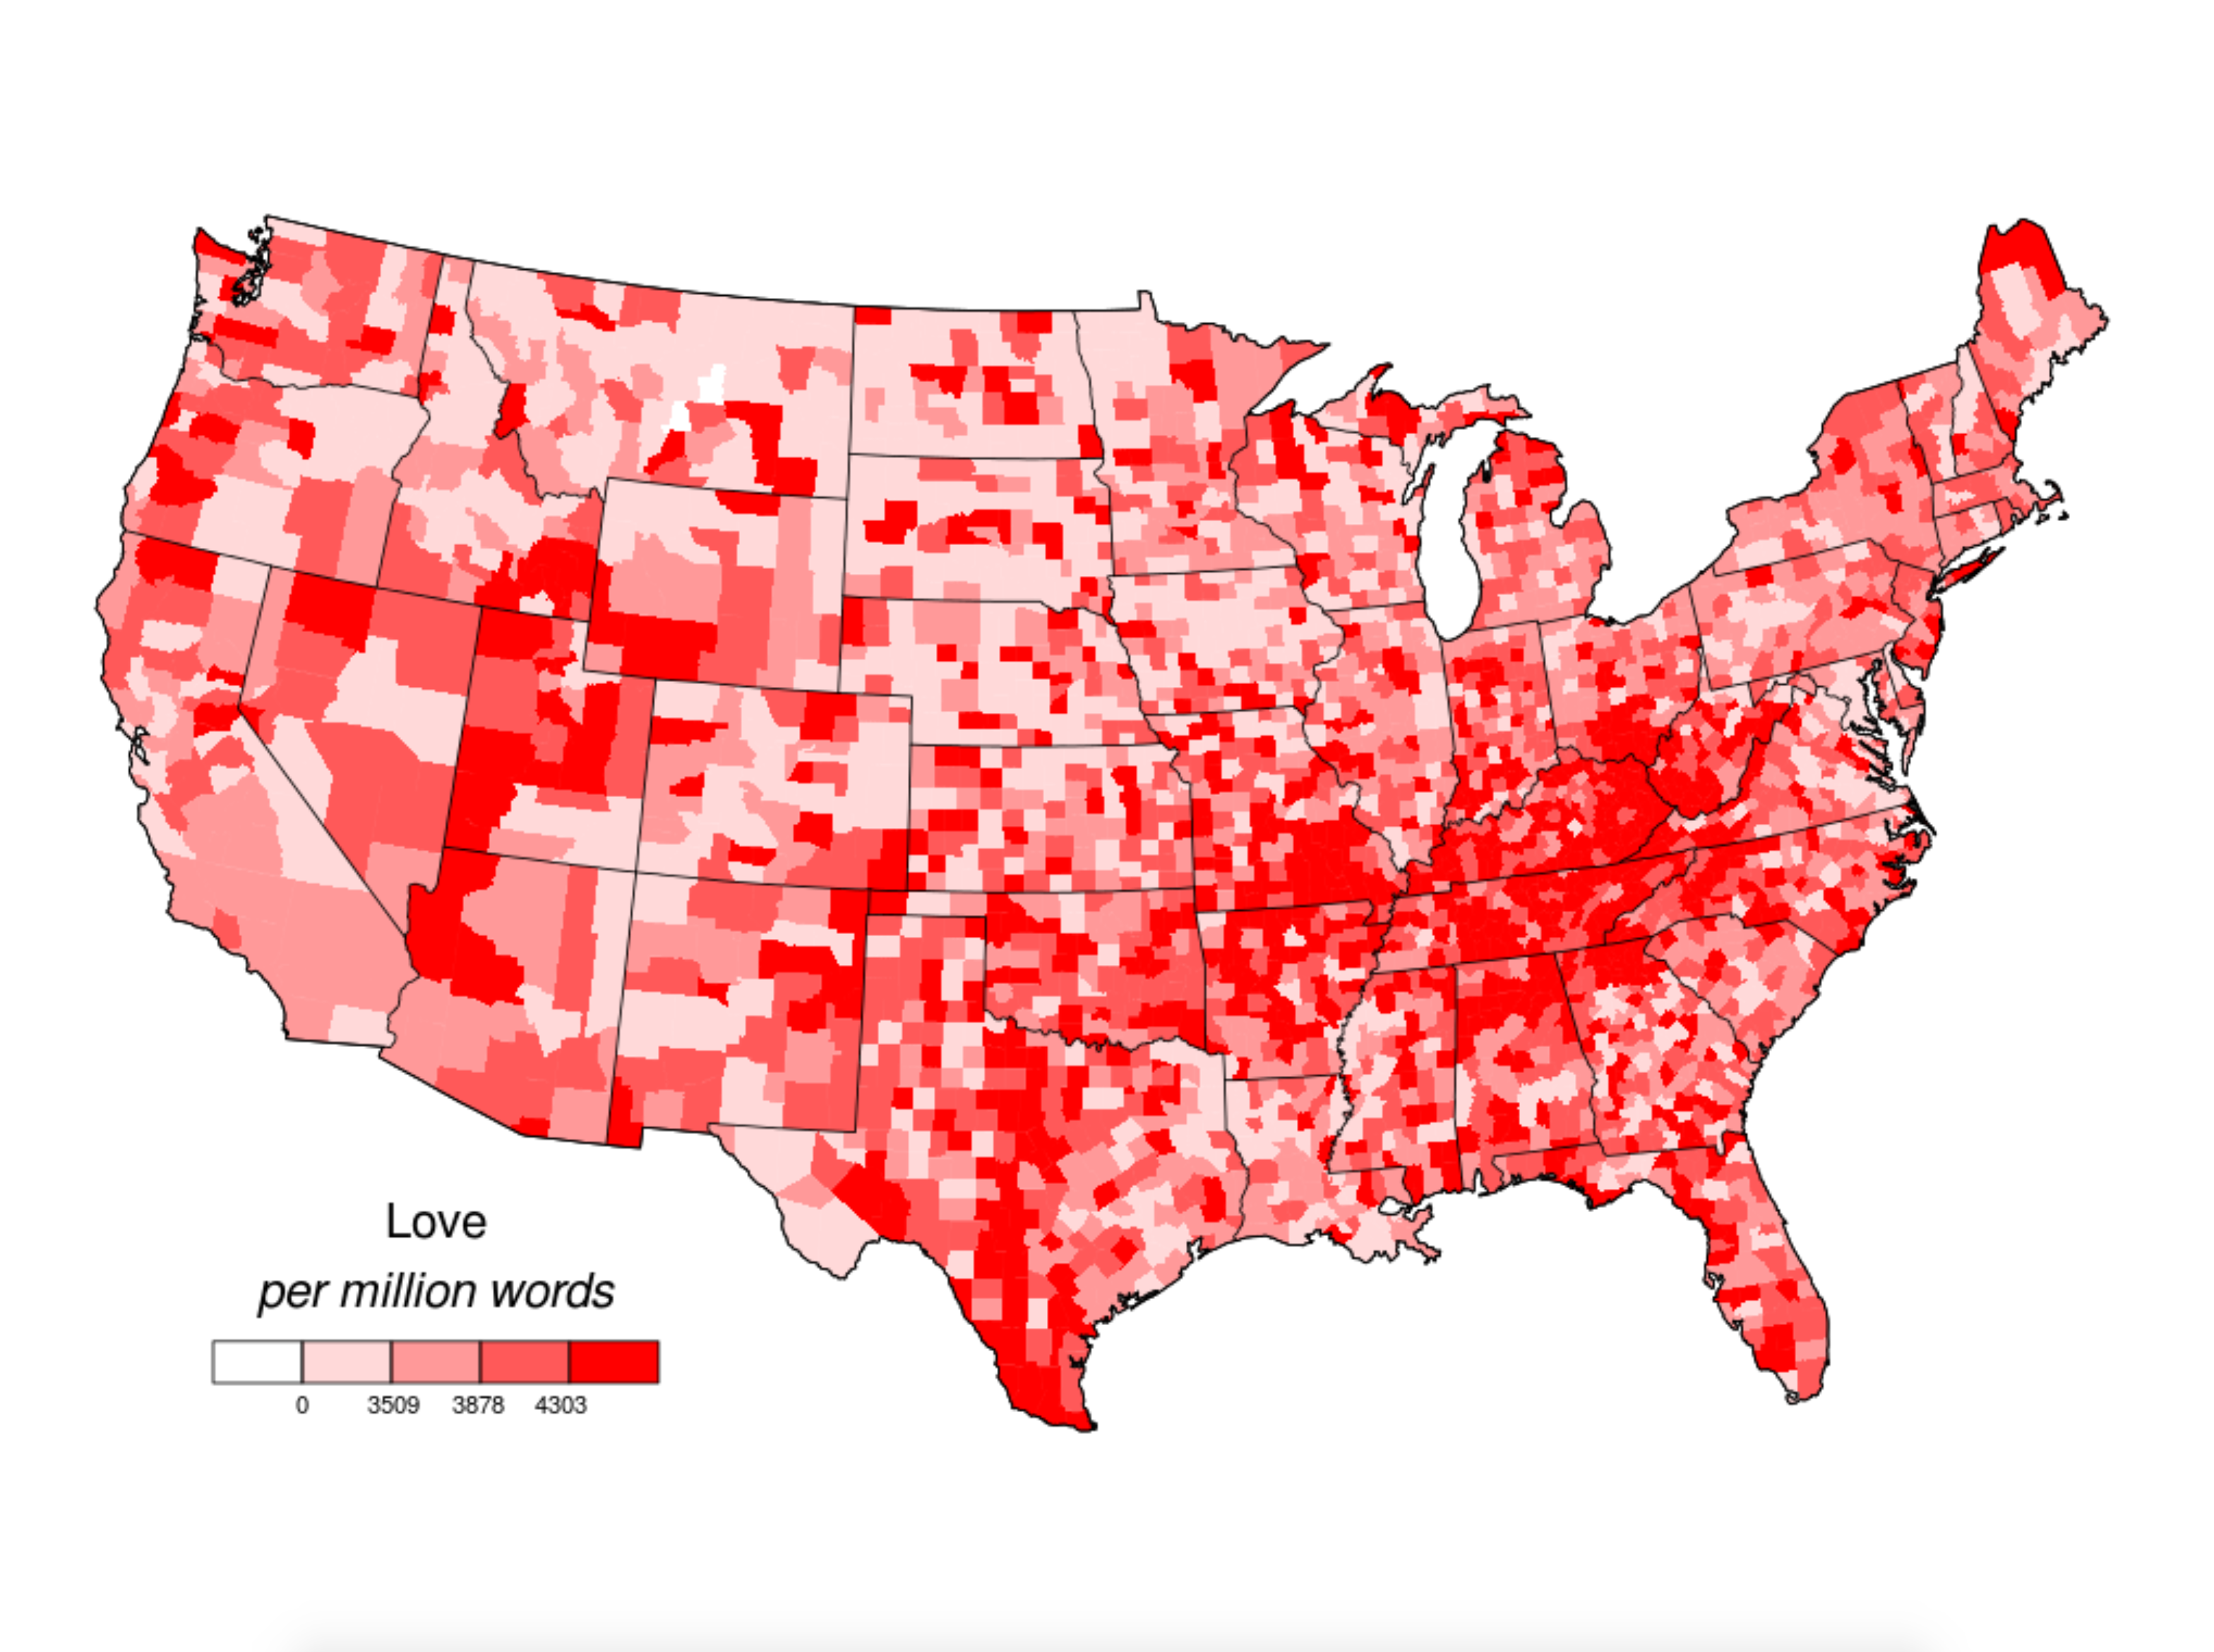
\includegraphics[width=0.9\textwidth]{geotaggedtweet.png} \\
\footnotesize source: Jack Grieve's talk \url{https://dl.dropboxusercontent.com/u/99161057/AMES3.pdf} 
\end{frame}

\begin{frame}
\frametitle{Why visualize?: Some application scenarios}
\framesubtitle{Plotting the process of reading a text}
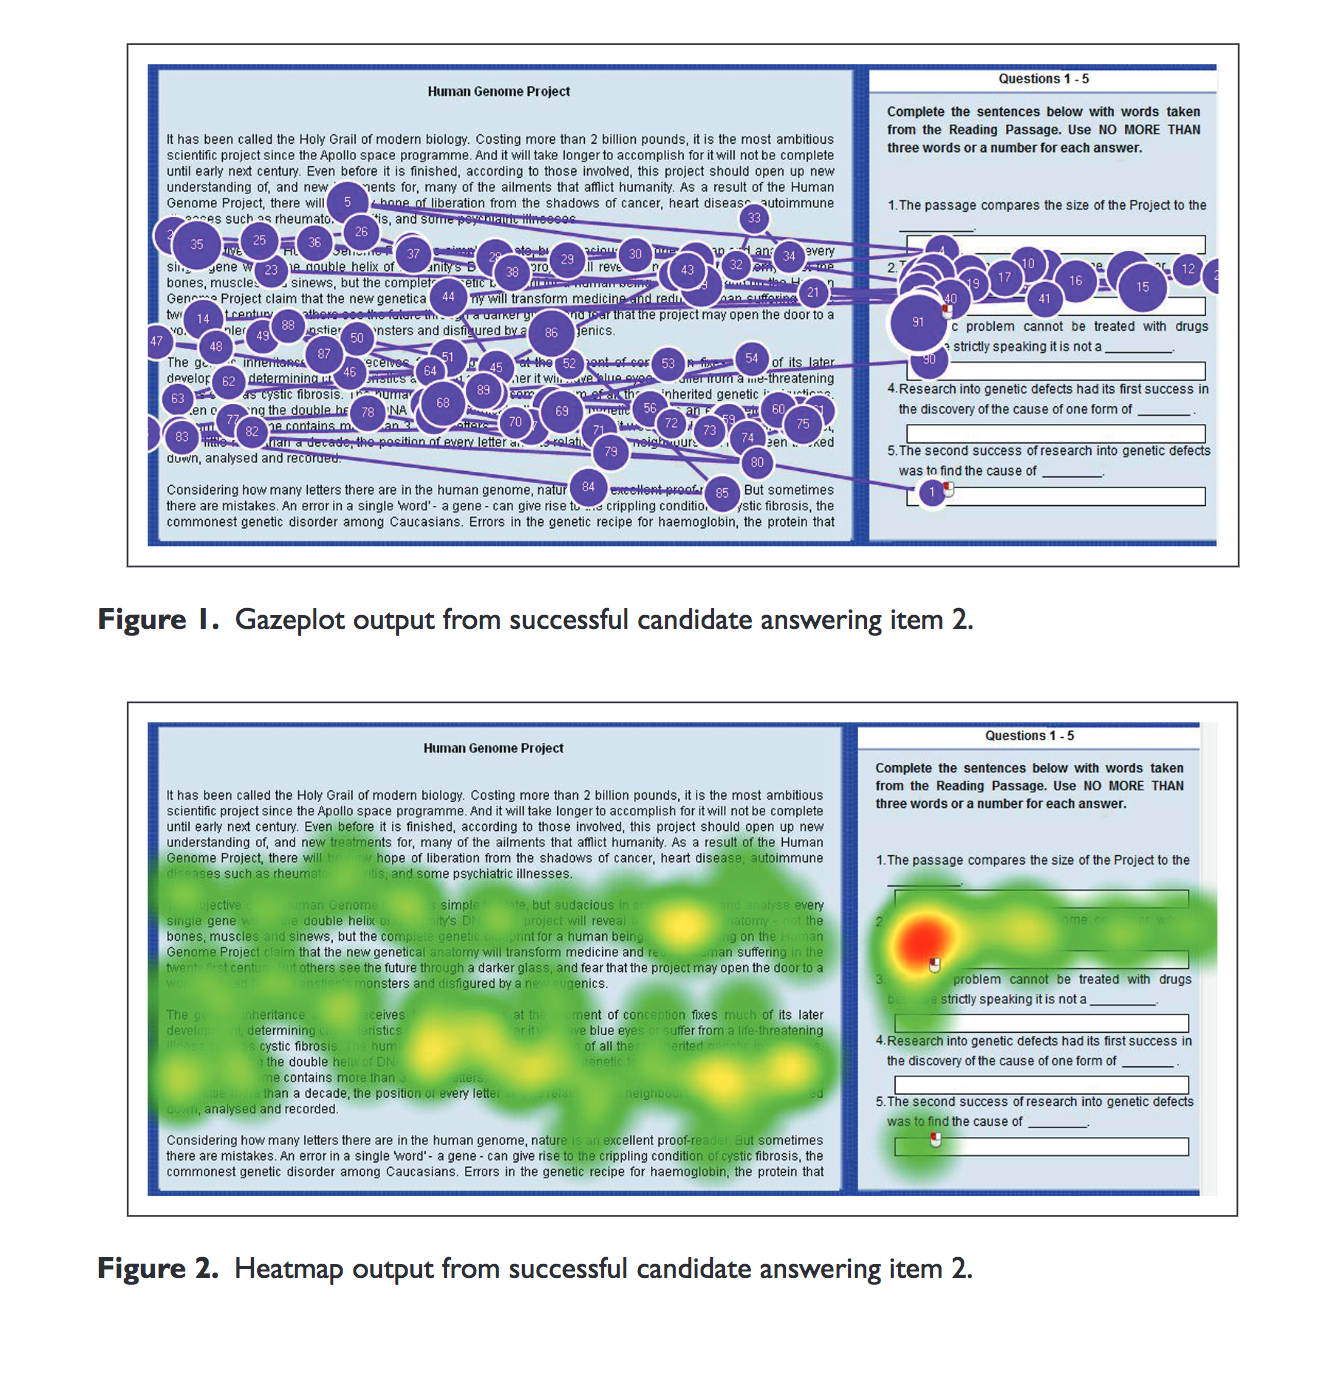
\includegraphics[width=0.65\textwidth]{textgazeplot.png} \\
\scriptsize source: \url{http://journals.sagepub.com/doi/abs/10.1177/0265532212473244} 
\end{frame}

\begin{frame}
\frametitle{Why visualize?: Some application scenarios}
\framesubtitle{Keyword in Context (KWIC)}
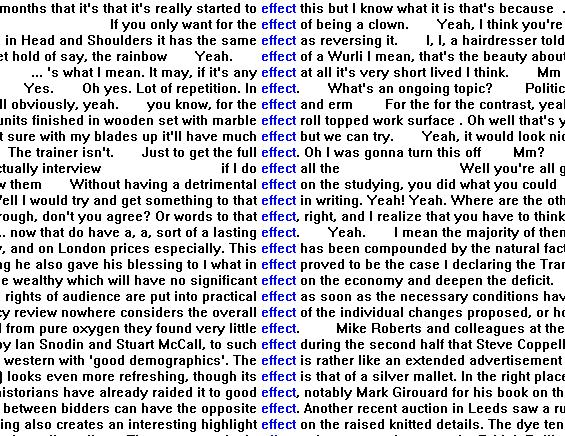
\includegraphics[width=0.8\textwidth]{kwic.jpeg} \\
\scriptsize source: \url{https://ota.ox.ac.uk/documents/searching/figure3.jpg} 
\end{frame}

\begin{frame}
\frametitle{Why visualize?: Some application scenarios}
\framesubtitle{Plotting word sequences - a word tree}
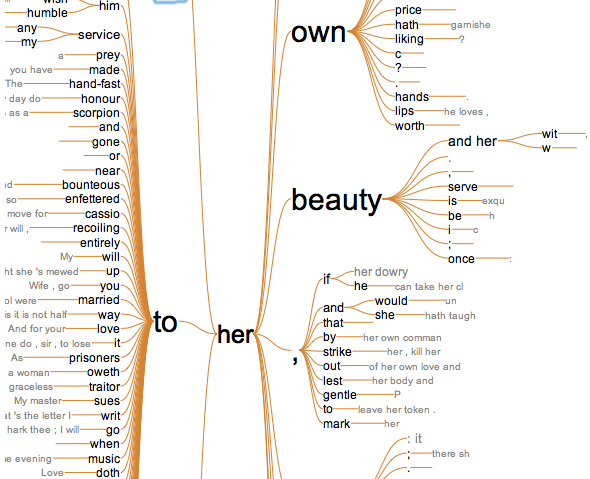
\includegraphics[width=0.8\textwidth]{word-tree.png} \\
\scriptsize source: \url{http://wordseer.berkeley.edu/files/2012/01/word-tree-her.png} 
\end{frame}

\begin{frame}
\frametitle{Why visualize?: Some application scenarios}
\framesubtitle{Visualizing sentiment-1}
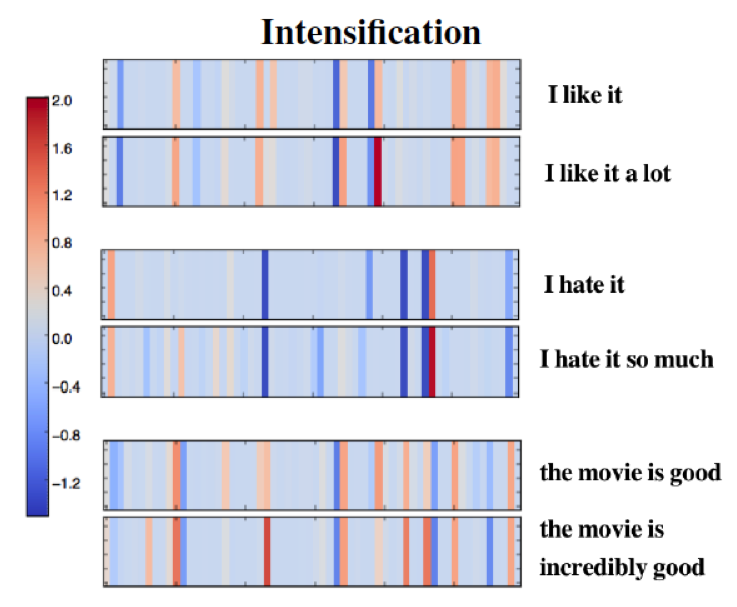
\includegraphics[width=0.8\textwidth]{nn-1.png} \\
\scriptsize source: \url{https://web.stanford.edu/~jurafsky/pubs/visualizing16.pdf} 
\end{frame}

\begin{frame}
\frametitle{Why visualize?: Some application scenarios}
\framesubtitle{Visualizing sentiment-2}
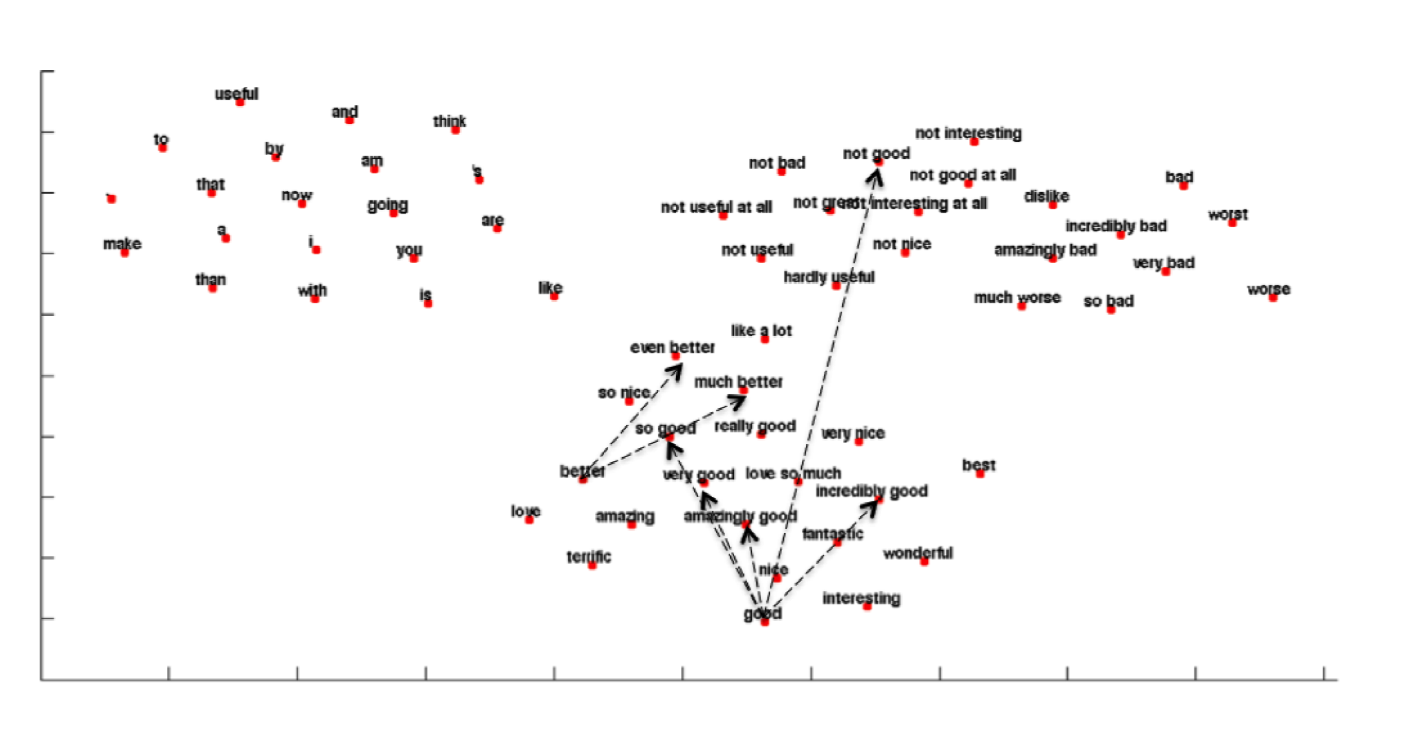
\includegraphics[width=0.99\textwidth]{nn-2.png} \\
\scriptsize source: \url{https://web.stanford.edu/~jurafsky/pubs/visualizing16.pdf} 
\end{frame}

\begin{frame}
\frametitle{Why visualize?: Some application scenarios}
\framesubtitle{Visualizing the discourse of a text}
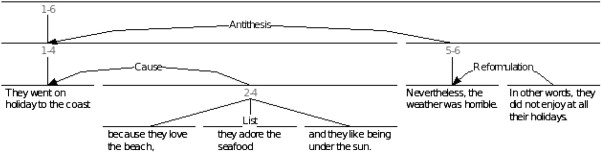
\includegraphics[width=0.99\textwidth]{discoursevisualization.jpeg} \\
\scriptsize source: \url{http://ars.els-cdn.com/content/image/1-s2.0-S0957417411009584-gr1.jpg} 
\end{frame}

\begin{frame}
\frametitle{Why visualize?: Some application scenarios}
\framesubtitle{Phrasenet}
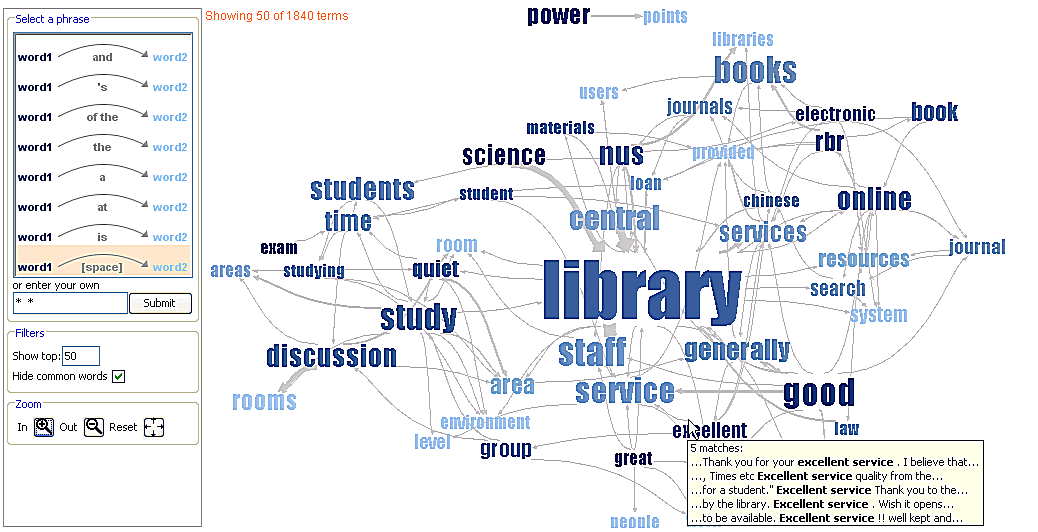
\includegraphics[width=0.99\textwidth]{phrasenet.png} \\
\scriptsize source: \url{http://blog.nus.edu.sg/aarontay/files/2009/03/manyeyesphrasenet.png} 
\end{frame}

\begin{frame}
\frametitle{Why visualize?: Some application scenarios}
\framesubtitle{Visualizing language change over time}
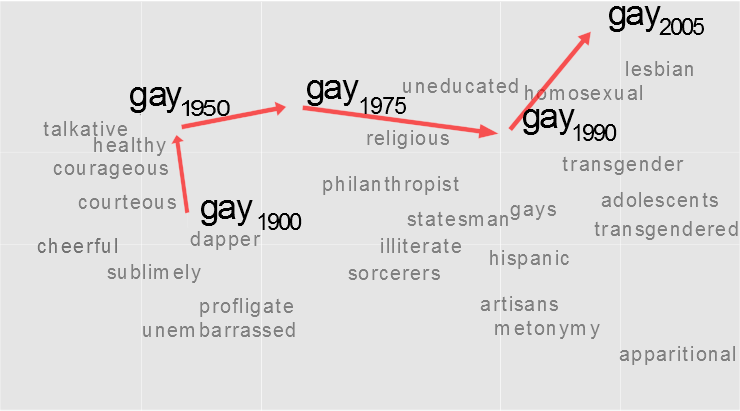
\includegraphics[width=0.99\textwidth]{gay_invisible.png} \\
\scriptsize source: \url{http://viveksck.github.io/langchangetrack/img/gay_invisible.png} 
\end{frame}

\begin{frame}
\frametitle{Stanford Dissertation Browser}
\url{https://nlp.stanford.edu/projects/dissertations/browser.html}
\end{frame}

\begin{frame}
\frametitle{Google Ngram viewer}
\url{https://books.google.com/ngrams}
\end{frame}

\begin{frame}
\frametitle{Docuburst/Starburst/ other such tools}
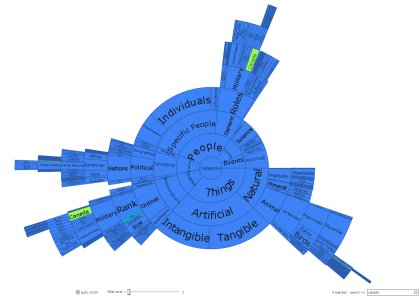
\includegraphics[width=0.99\textwidth]{docuburst.jpeg}
\\ \scriptsize \url{http://vialab.science.uoit.ca/wp-content/uploads/2011/12/starburstdemo.jpg}
\end{frame}

\begin{frame}
\frametitle{Some visualizations we already saw}
\begin{itemize}
\item Frequency plots
\item Dispersion plots
\item Word clouds
\end{itemize}
(Anything else you can think of?)
\end{frame}
%Some other visualizations we saw in the past - e.g., topic model visualization examples.

\begin{frame}
\frametitle{Challenges of text visualization}
\begin{itemize}
\item What do we want from the visualization? \pause
\\ e.g., word clouds don't tell us about structure. So, if we want to know beyond words, it is perhaps not useful. \pause
\item How should we represent the data to get the visualization?
\item What kind of pre-processing of text is needed? What kind of language processing tools do I need?
\item What kind of visualization tools are needed?
\item How much to put on the visual? Screen size, colors, layout etc.
\end{itemize}
\end{frame}

\begin{frame}
\frametitle{Pre-processing needed for visualization}
\begin{itemize}
\item sentence splitting
\item word splitting (may be: stemming, lower casing, removing stopwords)
\item POS tagging of words
\item recognizing person/location names, identifying temporal expressions etc.
\item Understanding the syntactic structure (if we want to derive - event information such as who did what to whom etc)
\end{itemize}
... depending on the need, there may be more processing.
\end{frame}

\begin{frame}
\frametitle{Visualizing visualization techniques}
\url{http://textvis.lnu.se/}
\\ Some recent research in this direction: \url{http://research.dbvis.de/text/}
\end{frame}

\begin{frame}
\frametitle{Text Visualization in R}
\begin{itemize}
\item We will work with "wordcloud" and "stylo" libraries in the class this week and next.
\item Other useful libraries for text visualization: qdap
\item Useful graph plotting libraries in R: ggplot2, dygraphs, plotly etc
\item Shiny - \url{https://shiny.rstudio.com/} is a web application framework for R. You can create interactive visualizations (for both textual and non-textual data).
\end{itemize}
\end{frame}

\begin{frame}
\frametitle{}
\centering
\Large Illustration of Stylo
\end{frame}

\begin{frame}
\frametitle{Assignment 6 description}
\begin{itemize}
\item Task: create visualizations using "wordcloud" package in R
\item Grade: 10\%
\item Deadline: 14 April 2018
\item Submission format: Doc or pdf report along with the R code you wrote.
\end{itemize}
\end{frame}

\begin{frame}
\frametitle{Initial report on your final project}
\begin{itemize}
\item Task: Idea for your final project, tasks involved, timeline etc. (max 2 pages, without double spacing)
\item Grade: 5\%
\item Deadline: 7 April 2018
\item Submission format: pdf
\end{itemize}
\end{frame}

\begin{frame}
\frametitle{Next class}
\begin{itemize}
\item Time to work with Mallet
\item Exercises related to creating visualizations
\item To do before next class:
\begin{itemize}
\item Skim through the two pdf files uploaded in this week's presentations folder. 
\item Install stylo library on your laptop if possible (those who work on their own machines)
\end{itemize}
\item Attendance question to be answered before Thursday's class: Write a quick summary of any one of the two articles.
\end{itemize}
\end{frame}

\end{document}

Useful refs.
http://courses.cs.washington.edu/courses/cse512/16sp/lectures/CSE512-Text.pdf
http://cs.smith.edu/dftwiki/index.php/Visualizations:_Lexical/Text
http://www.cs171.org/2015/assets/slides/12-TextVis.pdf
http://www.springer.com/us/book/9789462391857
http://textexture.com/
http://research.dbvis.de/text/
http://guides.library.duke.edu/text_analysis/text_vis
http://textvis.lnu.se/
http://hci.stanford.edu/courses/cs448b/f11/lectures/CS448B-20111117-Text.pdf
http://citeseerx.ist.psu.edu/viewdoc/download?doi=10.1.1.695.6751&rep=rep1&type=pdf
